\section{Memory Decoding}
\label{sec:memory-decoding}

\subsection{Internal Construction}
\label{subsec:internal-construction}

The internal construction of a RAM of $m$ words and $n$ bits per word consists of $m \times n$ binary storage cells and associated decoding circuits for selecting individual words. The binary storage cell is the basic building block of a memory unit. The equivalent logic of a binary cell that stores one bit of information is shown in Fig. 5.
\begin{figure}[H]
  \centering
  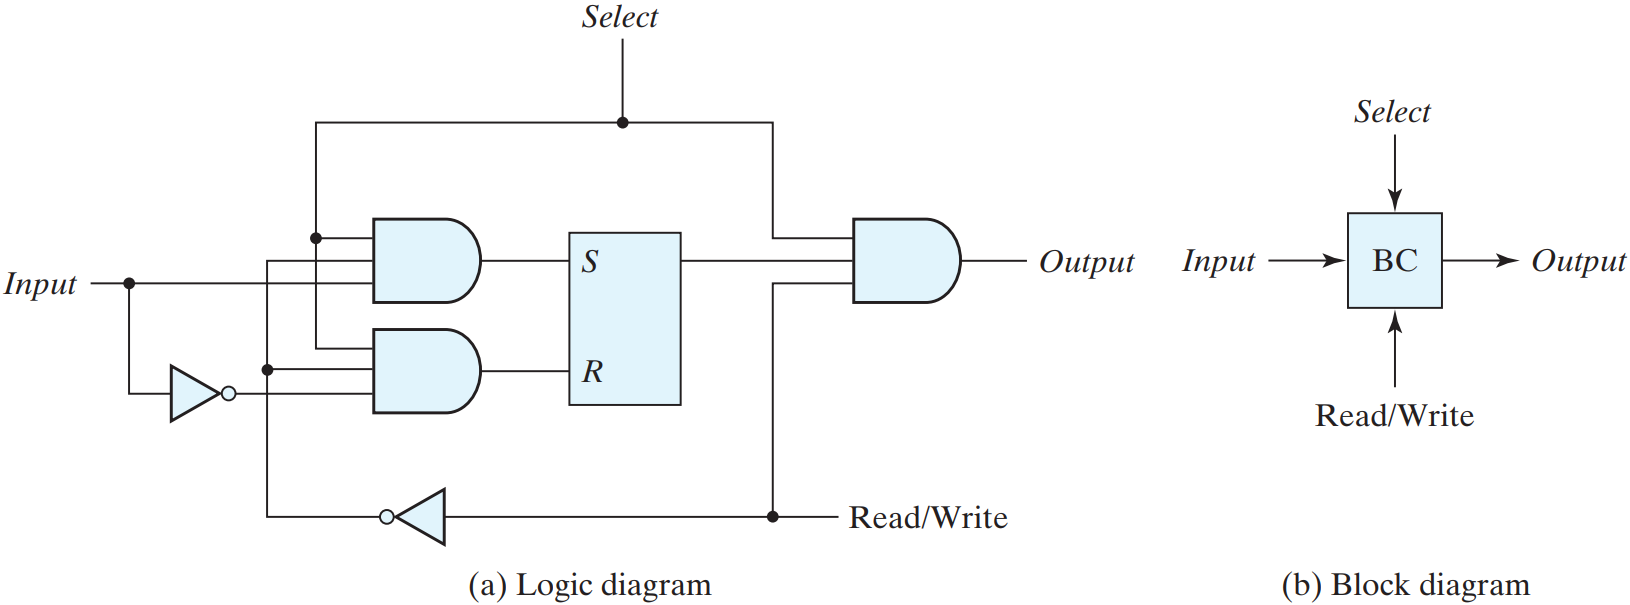
\includegraphics[width=\linewidth]{img/fig-7.5.png}
  \caption{Memory cell}
  \label{fig:7.5}
\end{figure}

\noindent The binary cell stores one bit in its internal latch.
\begin{itemize}[leftmargin=0.6cm]
  \item The select input enables the cell for reading or writing
  \item The read/write input determines the operation of the cell when it is selected.
    \begin{itemize}[leftmargin=0.6cm]
      \item \textit{Read}: A 1 in the read/write input provides the read operation by forming a path from the latch to the output terminal.
      \item \textit{Write}: A 0 in the read/write input provides the write operation by forming a path from the input terminal to the latch.
    \end{itemize}
\end{itemize}

\vspace*{\fill}
\columnbreak

\noindent The logical construction of a small RAM is shown in Fig. 6.
\begin{figure}[H]
  \centering
  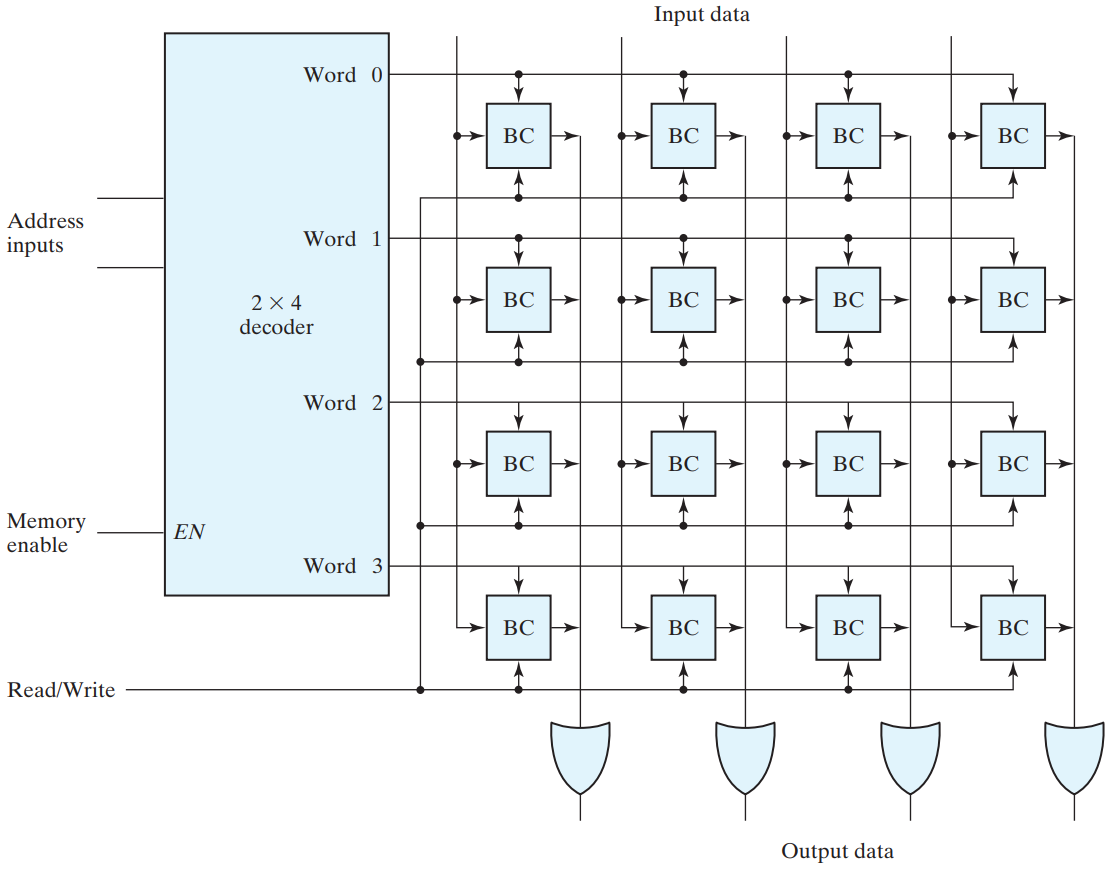
\includegraphics[width=\linewidth]{img/fig-7.6.png}
  \caption{Diagram of a $4 \times 4$ RAM}
  \label{fig:7.6}
\end{figure}

A memory with $2^k$ words of $n$ bits per word requires $k$ address lines that go into a $k \times 2^k$ decoder. Each one of the decoder outputs selects one word of $n$ bits for reading or writing.

\subsection{Coincident Decoding}
\label{subsec:coincident-decoding}

A decoder with $k$ inputs and $2^k$ outputs requires $2^k$ AND gates with $k$ inputs per gate. The total number of gates and the number of inputs per gate can be reduced by employing two decoders in a two-dimensional selection scheme. In this configuration, two $k/2$-input decoders are used instead of one $k$-input decoder: One decoder for row selection, one decoder for column selection.

The two-dimensional selection pattern is demonstrated in Fig. 7 for a 1K-word memory. Instead of using a single $10 \times 1,024$ decoder, we use two $5 \times 32$ decoders. The five most significant bits of the address go to input $X$ and the five least significant bits go to input $Y$.

\begin{figure}[H]
  \centering
  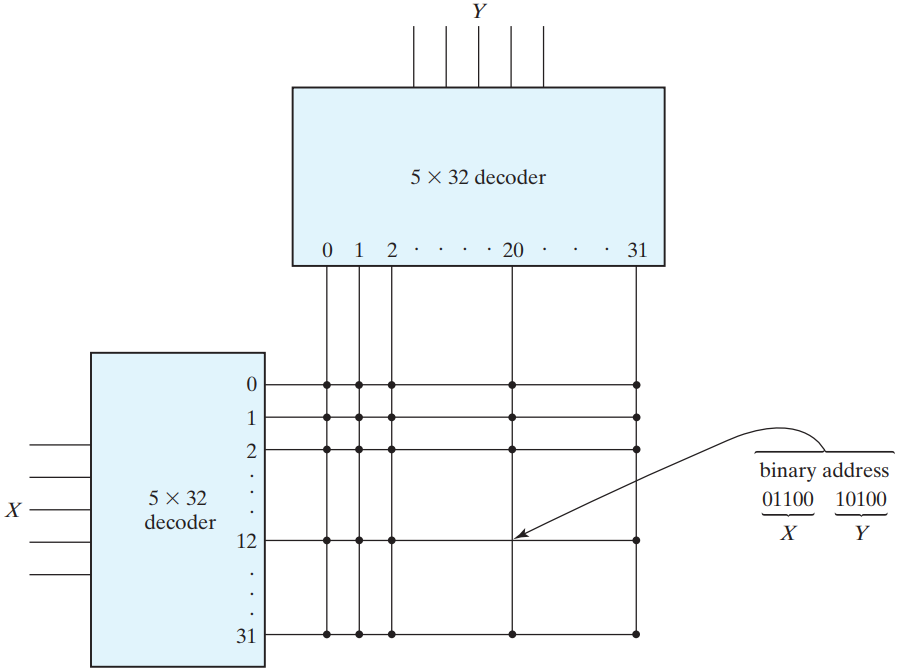
\includegraphics[width=\linewidth]{img/fig-7.7.png}
  \caption{Two-dimensional decoding structure for a 1K-word memory}
  \label{fig:7.7}
\end{figure}

\vspace*{\fill}
\columnbreak

\subsection{Address Multiplexing}
\label{subsec:address-multiplexing}

Because of their simple cell structure, \textit{DRAMs typically have four times the density of SRAMs}. This allows four times as much memory capacity to be placed on a given size of chip. The cost per bit of DRAM storage is three to four times less than that of SRAM storage. A further (operational) cost savings is realized because of the lower power requirement of DRAM cells. 

These advantages make DRAM the preferred technology for large memories in personal digital computers. DRAM chips are available in capacities from 64K to 512M bits. Most DRAMs have a 1-bit word size, so several chips have to be combined to produce a larger word size.

Because of their large capacity, the address decoding of DRAMs is arranged in a two-dimensional array, and larger memories often have multiple arrays. In a two-dimensional array, the address is applied in two parts at different times, with the row address first and the column address second.

We will use a 64K-word memory to illustrate the address-multiplexing idea. A diagram of the decoding configuration is shown in Fig. 8.

\begin{itemize}
  \item There is a single data input line, a single data output line, and a read/write control
  \item There are an eight-bit address input and two address strobes, the latter included for enabling the row and column address into their respective registers.
  \item The row address strobe (RAS) enables the eight-bit row register, and the column address strobe (CAS) enables the eight-bit column register. The bar on top of the name of the strobe symbol indicates that the registers are enabled on the zero level of the signal.
\end{itemize}

\vspace*{\fill}
\columnbreak

\begin{figure}[H]
  \centering
  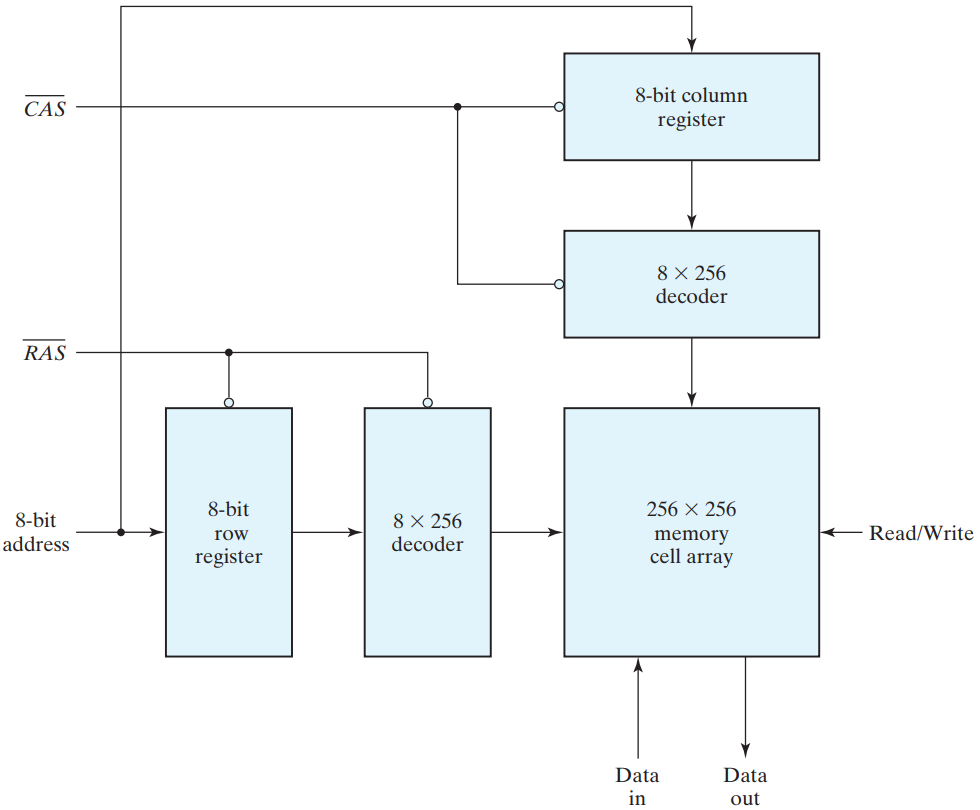
\includegraphics[width=\linewidth]{img/fig-7.8.png}
  \caption{Address multiplexing for a 64K DRAM}
  \label{fig:7.8}
\end{figure}